% !TEXroot=main.tex

\section{Grundlagen}
{
	Das Projekt baut auf einige Prinzipien, Algorithmen und Prozesse auf, welche im Folgenden kurz erläutert werden.
	\subsection{ROS}
	{
		Wie es jedermann von seinem Heimcomputer kennen, so gibt es auch für Roboter ein Betriebssystem. Analog unterstützt ROS, das Robot Operating System, auch bei der Bedienung und soll im folgenden kurz erklärt werden.		\subsubsection{Überblick}
		{
			Das sogenannte Robot Operating System, kurz ROS genannt, ist ein Open-Source Betriebssystem für Roboter, welches viele Tools und Software-Bibliotheken bietet. Die Entwicklung von ROS begann 2007 im Stanford Artificial Intelligence Laboratory. Ab 2009 wurde ROS im Institut Willow Garage fortgeführt,\parencite{Quigley09} bis ROS ab 2012 von der OSRF (Open Source Robotic Foundation) unterstützt wird. Seit der Veröffentlichung von ROS gibt es regelmäßig Updates und neuere Versionen von ROS, welche hauptsächlich mit Betriebssystem Linux, aber auch Windows oder MacOS kompatibel sind. 
			
			Die grundsätzliche Idee von ROS ist, alle Vorteile von vergleichbaren Produkten zu vereinen, während die Nachteile der jeweiligen Produkte behoben werden. Die Hauptbestandteile von ROS sind: Hardwareabstraktion, Gerätetreiber, Nachrichtenaustausch zwischen Programmen und Programmteilen und die Paketverwaltung. Alle diese Bestandteile sorgen dafür, dass der Roboter einfacher auf Daten zugreifen kann. Es handelt sich dabei um den aktuellen internationalen Standard, welcher auf den meisten Systemen einwandfrei läuft und dabei wenig Leistung beansprucht. Ein Gerätetreiber ist ein Programm, welches die Interaktion mit angeschlossenen, eingebauten oder virtuellen Geräten steuert. Beim Nachrichtenaustausch werden Nachrichten zum Empfänger versendet, bei welchen es sich um Signale oder Datenpakete handeln kann. Die Paketverwaltung hilft bei der Verwaltung von Software, die in Form von Programmpaketen vorliegt. Ein weiteres Ziel von ROS ist, oft wiederverwendbare Funktionen zugänglich zu machen. 
			
		}
		
		\subsubsection{Aufbau}
		{ 
			Programme werden in ROS als Pakete implementiert. Ein Paket besteht aus einer Manifestdatei, welche Metadaten (z.B. den Autor) über das Paket beinhaltet, sowie ausführbaren Skripten (Programmen). Pakete werden meist unabhängig voneinander entwickelt, können doch miteinander kommunizieren (siehe Datenaustausch). Pakete können (ähnlich zu Apps auf einem Handy) einzeln installiert bzw. deinstalliert werden, wobei einige Pakete andere benötigen, um zu funktionieren. Die Programme werden meist in den Programmiersprachen C++ oder Python geschrieben, welche beide die größte Integration in das ROS vorweisen.
			
			Der ROS-Core ist der Mittelpunkt des Betriebssystems. Dieses Programm steuert alle Vorgänge und sorgt dafür, dass Daten an korrekte Nodes weitergegeben werden, sowie vieles mehr. 
			
			Eine Grundkomponente von ROS sind sogenannte Nodes (Knotenpunkte), welche von Programmen initiiert werden können: Jeder dieser Nodes hat eine gewisse Funktion (z.B. das ansteuern von Motoren). Diese Knotenpunkte sind des Weiteren austauschbar, sodass es für verschiedene Motorenmodelle beispielsweise andere Nodes gibt, welche jedoch alle die gleiche Funktion erfüllen, nämlich das ansteuern der Motoren.
		}
	
		\subsubsection{Vorteile}
		{
			Der größte Vorteil des ROS ist die Aufteilung des Systems in universelle Komponenten. Der Datenaustausch der Komponenten ist standardisiert, \dahe die Daten, welche beispielsweise an Motoren weitergegeben werden, haben immer die gleiche Form. Dadurch können Hersteller für ihre Motoren Programme entwickeln, denn die Daten, welche an die Komponente zur Motorensteuerung weitergegeben werden. Gleiches gilt auch für die Ausgabe von Daten durch einzelne Komponenten. Diese Standardisierung von Daten erlaubt eine Flexibilität in der Spezifität der einzelnen Komponenten und erlaubt eine einfache Integration. Dadurch wird eine Kollaboration vieler Menschen überall auf der Welt ermöglicht. Forschungsergebnisse, wie \zb GMapping, worauf später eingegangen wird, werden damit für jedermann verfügbar und können leicht in die eigenen Systeme eingebunden werden.
		}
		
		\subsubsection{Datenaustausch}
		{
			Der Austausch von Daten kann sich als Graph vorgestellt werden. Jeder Knotenpunkt kann Daten aussenden oder empfangen. Der Datentyp, welcher ausgetauscht wird, kann beliebig bestimmt werden, jedoch beruht alles auf vier Grundtypen.
			\begin{itemize}
				\item Ganzzahlen (Integer)
				\item Kommazahlen (Float)
				\item Zeichen (Char)
				\item Ja\,/\,Nein (Boolean)
			\end{itemize}
			Basierend auf diesen Grundtypen können neue Datentypen gebaut werden. So kann man beispielsweise sagen, dass der Datentyp Auto
			\begin{itemize}
				\item eine Kommazahl hat, welche den Füllstand beschreibt,
				\item eine ganze Zahl hat, welche die Anzahl an Passagieren beschreibt,
				\item ein aus mehreren Zeichen bestehendes Kennzeichen hat,
				\item einen Ja\,/\,Nein-Wert hat, welcher bestimmt, ob der Motor an ist,
			\end{itemize}
			
			hat. Die Datenstruktur der ausgetauschten Daten wird Nachricht genannt. Nodes tauschen also Nachrichten untereinander aus. Jede Nachricht bekommt eine sogenannte Topic, was die Nachricht und deren Struktur eindeutig identifiziert. Ein Beispiel hierfür ist das \emph{cmd\textunderscore vel} Topic, welche Nachrichten des Types \emph{geometry\textunderscore msgs/Twist} weitergibt. Diese Daten geben Informationen über die aktuelle Bewegungsrichtung wieder. Zur Vereinfachung werden nur die Richtungen der Bewegung im 3D-Raum, nicht aber der Drehung, da diese für das Verständnis nicht notwendig ist, gezeigt. Die Struktur der Nachricht sieht daher (in gekürzter Fassung folgendermaßen aus:
			\newline
			
			linear:
			\begin{itemize}
				\item float64 x
				\item float64 y
				\item float64 z
			\end{itemize}
			
			\emph{float64} stellt in der Programmierung eine 64 Bit große Gleitkommazahl dar. Daraus folgt, dass diese Nachricht drei Zahlen für jede Richtung hat, woraus sich die Bewegungsrichtung des Roboters ergibt. Im Falle meiner Navigation ist die $z$-Koordinate irrelevant, da der Roboter sich nicht nach oben/unten bewegt, sondern nur auf der zweidimensionalen Ebene.
		}
		
		\subsubsection{Publisher-Subscriber}
		{
			Nodes sind von Programmen initiierte Knotenpunkte, auf welche das Programm, welches sie initiiert hat, Zugriff hat. Über diese Punkte können Daten bereitgestellt werden, indem das Programm diese publiziert (Publisher). Dies kann man sich wie ein Forum darstellen, in welchem eine Person mit einem Megafon die Daten verkündet. Andere Nodes (Listener/Subscriber) können diesen Punkt nun abonnieren, was bedeutet, dass die Daten an sie weitergeleitet werden. Diese Listener-Nodes sind vergleichbar mit Personen, die einem Forum betreten und daher alles hören, was der Redner (Publisher-Node) sagt. Bei dieser Variante des Datenaustausches bestimmt der Publisher, wann Daten verbreitet werden. Mehrere Listener-Nodes können ein Publisher-Topic abonnieren.
		}
		\subsubsection{Services}
		{ 
			Services bilden das Gegenstück zum Publisher-Subscriber-Modell. Hierbei stellt ein Node Aufgaben bereit, welche er auf Anforderung erfüllt. Node A bietet beispielsweise an, die Lichter in einem Raum an bzw. auszuschalten. Node B kann in diesem Fall auf den Service "Ändere Lichtzustand" von Node A zugreifen, woraufhin Node A das Licht an bzw. ausschaltet. Ohne Aufruf führt Node A dies jedoch nicht durch. Dies zeigt, dass bei diesem Modell nicht der Node, welche einen Service bereitstellt, den Zeitpunkt der Ausführung definiert, sondern ein anderer Punkt, welcher den Service aufruft.
		}
		
		\subsubsection{Visualisierung des Datenaustausches}
		{
			Der Datenaustausch zwischen verschiedenen Nodes kann mit Hilfe einfacher Tools visualisiert werden. Ein sehr wichtiges Tool ist \emph{rqt\textunderscore Graph}, welches alle Knoten und deren Kommunikationsbeziehungen als Graphen anzeigt. Dabei werden Nodes als Ellipsen und deren Verbindungen als Pfeile angezeigt. Verbindungen werden mit dem Namen des Topic, welches die Daten, welche Übertragen werden, beschreibt, beschriftet. Dies ist vereinfacht in Abbildung \ref{pic:rqt_graph_simplified} dargestellt. Hierbei veröffentlicht der Node \emph{number\textunderscore publisher} Daten auf dem Topic \emph{/number} an den Node \emph{number\textunderscore subscriber} (rechts), welche das Topic abonniert hat.
			
			\begin{figure}
				\centering
				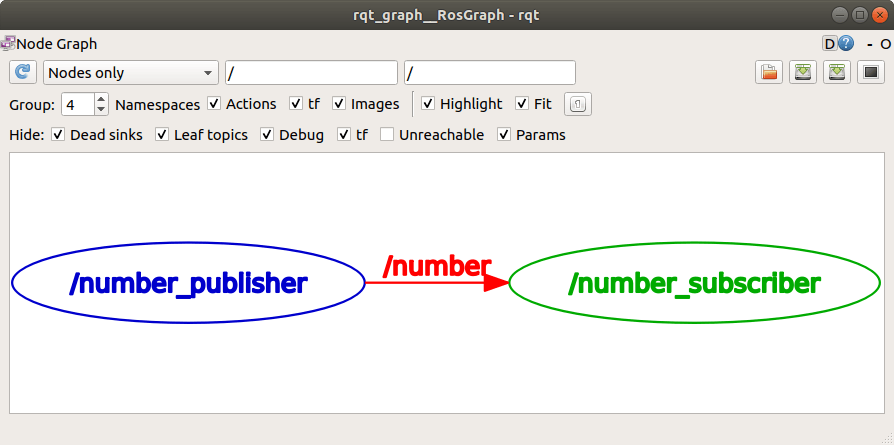
\includegraphics[height=5cm]{Bilder/rqt_graph_simplified.png}
				\caption{Ein vereinfachter Graph \\
					\parencite{rqtgraphsimplified1}} 
				\label{pic:rqt_graph_simplified}
			\end{figure}
		}
		
		\subsubsection{Drahtlose Übertragung}
		{ Wie bereits erwähnt, besitzt der Turtlebot einen Raspberry Pi. Dieser besitzt zwar für seine Größe vergleichsweise viel Leistung, jedoch wäre es natürlich vorteilhaft, die Rechenleistung eines herkömmlichen Desktop-PCs zu nutzen. Genau deshalb ermöglicht es das ROS, über mehrere Geräte hinweg zu kommunizieren. Das Herzstück bildet hierbei das ROS-Core Programm, welches alle Vorgänge innerhalb des Systems steuert. Dieses Programm muss auf einem der miteinander kommunizierenden Geräte aktiv sein. Mit Hilfe der IP-Adressen \footnote{Ähnlich einer Adressanschrift: Zahlenkombination zur eindeutigen Identifikation eines Gerätes in einem Netzwerk} der Geräte kommunizieren die Teilnehmer untereinander in einem Netzwerk, als ob alle Nodes auf einem Gerät ausgeführt werden würden. Dies ermöglicht das ausführen von Rechenintensiven Programmen auf einem Computer, während kleinere Programme, sowie der ROS-Core auf dem Turtlebot laufen. Das Gerät, auf welchem der Ros-Core läuft, wird auch ROS-Master genannt. Um beide Geräte zu verbinden, benötigt es nur wenige Einstellungen. Nachdem beide Geräte sich im gleichen Netzwerk befinden müssen die Parameter: \textbf{ROS\textunderscore IP} und \textbf{ROS\textunderscore Master \textunderscore URI} eingestellt werden. Ersterer beschreibt die IP-Adresse des Gerätes (für beide Geräte unterschiedlich) und letzterer Parameter beschreibt die IP-Adresse des ROS-Masters (für beide gleich, in meinem Fall ist es die Ip-Adresse des Turtlebot). Durch das ROS bauen beide Geräte eine Verbindung miteinander auf und kommunizieren miteinander.
			
		\begin{figure}[H]
			\centering
			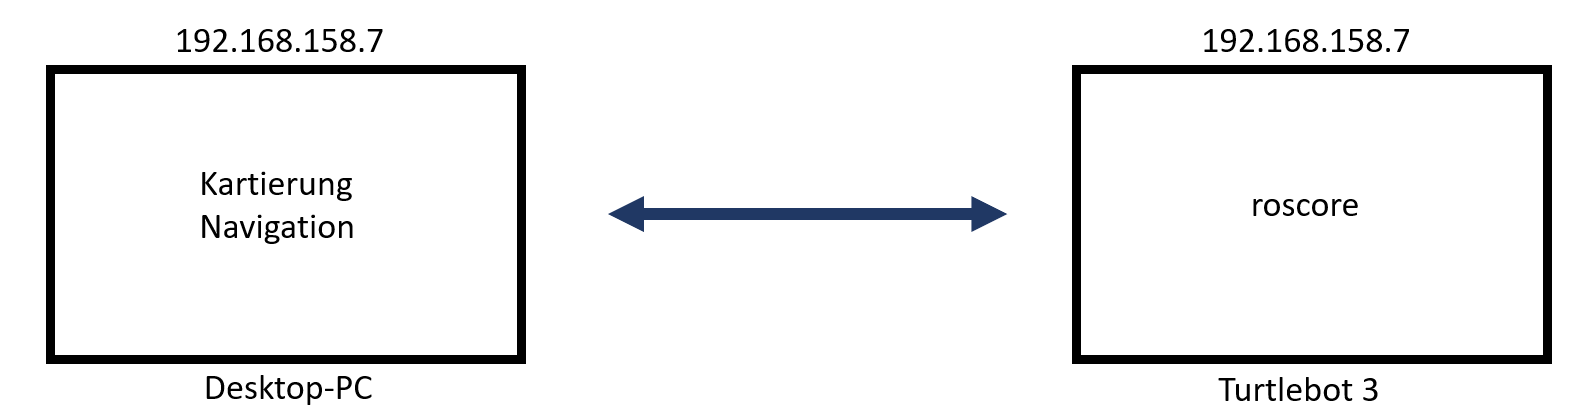
\includegraphics[height=4cm]{Bilder/network_turtlebot.png}
			\caption{Netzwerkverbindung und Programmaufteilung} 
			\label{pic:networkturtlebot}
		\end{figure}
		}
		
		\subsubsection{Simulation und Visualisierung}
		{
			Gazebo ist ein Open-Source-Programm\footnote{Frei zur Verfügung gestellt}, welches eine vollständige Simulation von Robotern, Umgebungen und Messungen ermöglicht. Robotermodelle können dazu modelliert werden, ebenso wie Umgebungen. Der Roboter kann sich daraufhin, wie in der realen Welt, bewegen und Messungen durchführen. Durch eine realistische Physik-Engine\footnote{Virtuelle Simulation physikalischer Kräfte} können Messungen wie in der echten Welt simuliert werden. D.\,h.\ der simulierte Roboter, in meinem Fall der Turtlebot, erhält Messdaten durch seinen Sensor, welche basierend auf der virtuellen Welt errechnet werden.Da ein großer teil der Entwicklubg zu Hause erfolgte, wurde dieses Programm oft genutzt, weshalb viele Abbildungen diesem Programm entstammen und nicht aus realen Experimenten.
			
			Rviz ist ebenso ein Open-Source-Tool, welches es ermöglicht, Daten, ob gemessen oder errechnet, zu visualisieren. Dafür empfängt ROS Daten der Nodes und präsentiert diese auf geeigneter Weise. So kann beispielsweise die Momentane Bewegungsrichtung als Pfeil, Messdaten des LiDAR-Sensors als Punkte oder eine Errechnete Karte als Hintergrundbild angezeigt werden
			
			
		}
	}
	\subsection{Turtlebot}
	{
		\subsubsection{Überblick}
		{
			Der Turtlebot ist ein beliebtes Robotermodell der Firma Robotis und kommt in verschiedenen Varianten. Das gute Preis-Leistungs-Verhältnis sowie die Einsteigerfreundlichkeit, kombiniert mit einer guten Integration in viele Programme, machen ihn zu einer guten Wahl für viele Projekte.
			Der Turtlebot 3 besteht aus vier Basisplatten, auf welchen die gesamte Technik des Roboters untergebracht ist. Auf der untersten Basisplatte findet man zwei Servomotoren der X-Series von Dynamixel vor, welche dem Turtlebot seine Mobilität verleihen, auf den anderen Plattformen ist ein Raspberry PI 3, welcher unter Umständen auch durch einen Raspberry Pi 4 ersetzt werden kann, sowie ein Einplatinencomputer vorzufinden. Bei Letzterem handelt es sich standardmäßig um einen Intel Joule 570x. Auf der obersten Basisplatte findet man Platz für einen Sensor vor, dort kann eine Kamera, allerdings auch ein Lasersensor oder ähnliches angebracht werden. Auf dem genutztem Turtlebot ist ein LiDAR-Sensor montiert. Dieser Sensor sendet Laserimpulse aus und kann durch das zurückgestrahlte Licht den Raum exakt vermessen. Der Roboter tastet die Umgebung mit den Laserimpulsen ab, was dazu führt, dass er Messpunkte erhält. 
			
			\begin{figure}[H]
				\centering
				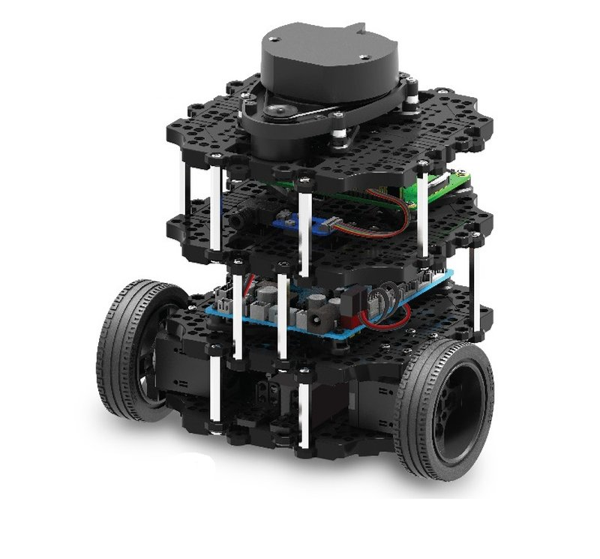
\includegraphics[height=5cm]{Bilder/turtlebot_3_burger.png}
				\caption{Der Turtlebot 3 in der "`Burger“ Variante} 
				\label{pic:turtle3burger}
			\end{figure}
			
			%Diese Messpunkte kann der Roboter als Wände oder andere Formen interpretieren. Allerdings handelt es sich dabei um eine 2D Messung, welche in unserem Fall die Umgebung des Roboters auf Höhe des Sensors scannt. Der Sensor kann sich unabhängig vom Roboter um 360° drehen. Ein Problem des Roboters ist, dass er mit dem Standard Sensor keine Hindernisse erkennt, welche nicht auf der Höhe des Sensors sind. Rundum vereint der Roboter eine exzellente Leistung bei günstigen Preisen.
		}
		
		\subsubsection{LiDAR-Sensor}
		{
			Ein LiDAR (Light detection and ranging) - Sensor, wie er auf der obersten Ebene des Turtlebot in Abbildung \ref{turtle3burger} zu sehen ist, sendet Laserimpulse aus und kann durch das zurückgestrahlte Licht den Raum exakt vermessen. Der Roboter tastet die Umgebung mit den Laserimpulsen ab, was dazu führt, dass er Messpunkte erhält. Diese Messpunkte kann der Roboter als Wände oder andere Formen interpretieren. Allerdings handelt es sich dabei um eine 2D-Messung, welche in unserem Fall die Umgebung des Roboters auf Höhe des Sensors scannt. Der Sensor kann sich unabhängig vom Roboter um 360° drehen. 
			Die Distanz eines Punktes ergibt sich aus der Zeitdifferenz zwischen Aussendung und Empfangen einer elektromagnetischen Welle (Licht) im infraroten Bereich.
			Der Entfernung wird wie folgt berechnet:
			
			\begin{equation}
				s = c \cdot \frac{t}{2}
			\end{equation} 
			Hierbei ist $s$ die Entfernung, $t$ die Zeit zwischen Aussendung und Empfangen, sowie $c$ die Lichtgeschwindigkeit.
			
			Ein Problem für Roboter ist, dass mit Hilfe des LiDAR-Sensor keine Hindernisse erkannt werden, welche nicht auf der Höhe des Sensors sind. Dies ist vor allem für größere Roboter ein Problem, kann aber aufgrund der Umgebung des Roboters, sowie aufgrund der höheren Labyrinth-Mauern vernachlässigt werden.
			\begin{figure}[H]
				\centering
				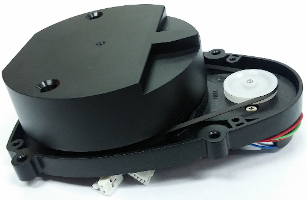
\includegraphics[height=5cm]{Bilder/lds_small.png}
				\caption{Der im Turtlebot 3 verbaute LiDAR-Sensor}
				\label{pic:lds_small}
			\end{figure}
		}
		
		\subsubsection{Raspberrry Pi}
		{
			Auf dem Turtlebot ist ein kleiner Computervom Typ Raspberry Pi verbaut. Standardmäßig handelt es sich dabei um das Modell der Reihe 3, welches jedoch aus Leistungsgründen mit einem Modell der 4. Generation ausgetauscht worden ist. Dieser Mikrocomputer stellt das Herzstück des Roboters dar und steuert alle Vorgänge. Wie ein jeder Computer besteht auch der Raspberry Pi aus einem Prozessor, Arbeitsspeicher, einer SD-Karte als nichtflüchtiger Speicher und vielem mehr. Zwar stellt die Firma Raspberry auch eine graphische Benutzeroberfläche bereit, jedoch ist diese zur Programmierung nicht notwendig und wird deshalb nicht verwendet, da diese Leistung verbraucht, welche für Berechnungen verwendet werden könnte. Aus diesem Grund wird der Raspberry Pi mit einem einfachen Betriebssystem, welches nur eine Konsole anzeigt, um Leistung zu sparen, verwendet.
		}
	}
	\subsection{Kartierung}
	{
		\subsubsection{SLAM}
		{
			SLAM (\emph{Simultaneous Localization and Mapping, dt.: Simultane Positionsbestimmung und Kartierung}) beschreibt den Prozess, in welchem eine Karte durch Messdaten erstellt wird, wobei der Roboter selbst auf der Karte verordnet wird.
			Im Fall des Turtlebot geschieht dies mithilfe der Messdaten des LiDAR-Sensors, welcher die Entfernung von Objekten durch Laserstrahlen misst (\emph{siehe LiDAR-Sensor})	
		}
		
		\subsubsection{Positionierung}
		{
			Der Roboter wird anfangs auf den Mittelpunkt der, zu Beginn noch nicht vorhandenen Karte, welche erst durch Messdaten entsteht, platziert. Dieser Punkt wird als Kartenursprung ($P(0|0)$ interpretiert). Die Position des Roboters wird entsprechend der Bewegung seiner Motoren kalkuliert. Mithilfe des Umfangs der Reifen kann die bewegte Distanz errechnet werden, da dem Roboter die Winkeländerung der Motoren, z.B. eine Drehung dieser um 180°, bekannt ist. Diese werden an die Motoren übermittelt, wobei die Information noch an andere Teile weitergeleitet werden kann, hier der Mikrochip auf der Hauptplatine des Raspberry Pi 3 in der Mitte der Roboters, welcher damit Rechnungen, eben zur Positionskorrektur durchführen kann. Vereinfacht gilt daher bei einer geraden Bewegung
			\begin{equation}
				D = R \cdot U
			\end{equation} 
			
			Hierbei steht $D$ für die zurückgelegte Distanz, $R$ für die Umdrehungen der Motoren und $U$ für den Umfang der Reifen. Die Rotation, also die Drehung des Roboters, wird aus der Rotationsdifferenz beider Motoren berechnet. Dreht sich der rechte Motor weiter (größerer Winkel), so dreht sich der Roboter nach links, für eine Rechtsdrehung gilt das Gegenteil.
			Auf diese Weise kann nur aus den Daten, welche an der Motoren gesendet wird, errechnet werden wie weit und in welche Richtung der Roboter sich bewegt hat.
			Die Raddrehungen werden aus den Motoren ausgelesen und entsprechend zu linearem Anteil und Rotationsanteil berechnet. Diese weichen durch Umwelteinflüsse und Messungenauigkeiten leicht von der Realität ab.
			
			
		\subsubsection{GMapping}
		{
			GMapping beschreibt einen SLAM-Algorithmus, welche an der Universität Freiburg über Jahre hinweg entwickelt worden ist. Dieser ist einer der  meist genutzten Algorithmen für diese Zwecke und deshalb gibt es auch eine Implementation für das Robot-Operating-System. Die Entwicklung eines eigenen Kartierungsalgorithmus geht weit über die Zeitspanne dieses Projektes hinüber, weshalb das GMapping-ROS-Paket verwendet wird (siehe \emph{Kartierung}) %https://people.eecs.berkeley.edu/~pabbeel/cs287-fa11/slides/gmapping.pdf
			
		}
	}

	\subsection{Monte-Carlo-Lokalisation}
	{ 
		Hat ein Roboter eine Karte seiner Umgebung. bringt diese ohne die Position des Roboters in der Karte nicht viel. Die Monte-Carlo-Lokalisation ist eine Möglichkeit, um die Position des Roboters innerhalb der Karte zu bestimmen.  Dafür wird die Karte der Umgebung sowie die Sensordaten benötigt. Anfangs ist es gleich wahrscheinlich, dass der Roboter sich in jeglicher Stelle auf der Karte befindet. Nun werden die gemessenen Sensorpunkte und die Karte der Umgebung übereinander gelegt. Stimmen Hindernisse, welche durch die Karte in der Nähe sind, sowie gemessene Sensordaten der realen Welt überein, so ist es wahrscheinlich, dass sich der Roboter an dieser Stelle in der Karte befindet. Misst der Turtlebot beispielsweise einen Runden Gegenstand vor sich und in einer Position auf der Karte ist in gleicher Distanz eine Runde Säule vor dem Roboter, so ist es wahrscheinlich, dass der Roboter sich in dieser Position befindet. Nachdem dieser sich bewegt hat, wird der Vorgang wiederholt, wodurch die möglichen Positionen immer nähe beieinander liegen, da entfernte Schätzungen aufgrund der vielseitigen Umgebung nicht mehr mit den Sensordaten übereinstimmen. 
	}
	\subsection{Wegfindung}
	{
		\subsubsection{Definition}
		{
			Pathfinding (\emph{dt. Wegfindung}) beschreibt den Prozess der Wegfindung, wobei der kürzestmöglichen Weg von einem Startpunkt zu einem Zielpunkt gefunden werden soll. Dieser Prozess setzt eine Karte der Umgebung (\emph{siehe SLAM}), in welcher ein Weg gefunden werden soll, voraus.
		}
		
		\subsubsection{Anwendung in der heutigen Welt}
		{
			Pathfinding-Prozesse sind von heutiger Technologie nicht mehr zu trennen. Sie sind überall präsent und helfen uns, auch wenn wir es manchmal nicht bemerken . Navigationssysteme müssen die kürzeste Route zu einem Zielpunkt finden, wohingegen Staubsaugroboter Orte in einem Haus erreichen müssen. Signale über Satelliten hinweg werden auch über den kürzesten Weg geleitet. Diesen zu finden bedeutet immer, dass für den Transport weniger Aufwand und Zeit benötigt wird
		}
		
		\subsubsection{Algorithmen zur Umsetzung}
		{
			Für die Wegfindung gibt es viele etablierte Algorithmen, jedoch stellt sich nun die Frage, welcher am Nützlichsten ist. Diese Nützlichkeit wird meist an zwei Faktoren gemessen. Diese sind zum einem die Genauigkeit, welche beschreibt, ob ein Algorithmus den besten Weg findet, und zum anderen die Geschwindigkeit. Diese beschreibt, wie effizient ein Algorithmus den idealen Weg findet. Mit Geschwindigkeit ist also nicht die Zeit der Ausführung gemeint, welche mit der Effizienz jedoch stark zusammenhängt, da diese je nach genutzten Bauteilen in Computern variiert. Vielmehr wird, wie erwähnt, die Rechenintensität als Maß genutzt. Diese beschreibt, wie viele Schritte durchgeführt werden müssen, bis der ideale Weg gefunden wurde. Je geringer, desto besser. 
			
			Viele Wegfindungsalgorithmen nutzen das gleiche Grundprinzip. Die Karte wird in kleine Vierecke unterteilt. Vom Startpunkt aus wird nun in eine Richtung gegangen und zwar einen Schritt weit. Dabei wird diese Stelle als "besucht" angesehen, wobei von ihr aus nun in weitere Richtungen gelaufen werden kann (Abbildung \ref{pic:pathfinding_procedure_1}). Grenzt eine besuchte Fläche an das Ziel an, so wurde ein Weg gefunden. Nachdem anfangs in jede Richtung ein Schritt in die Tiefe gegangen wurde, wird nun erneut in eine andere Richtung gegangen, bis in jede Richtung ein Schritt gegangen bzw. abgesucht worden ist (Abbildung \ref{pic:pathfinding_procedure_4}). Eine Tiefe (Längeneinheit) wurde somit vollständig abgedeckt. Daraufhin wird nun das Gleiche mit einer Tiefe von zwei zum Startpunkt hin wiederholt wird.
			
			\begin{figure}[H]
				\captionsetup{width=.8\linewidth}
				\centering
				\begin{subfigure}[h]{.17\linewidth}
					\centering
					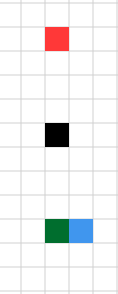
\includegraphics[scale=0.6, height =4cm]{Bilder/pathfinding_procedure_1.png}
					\subcaption{1. Feld durchlaufen}
					\label{pic:pathproc1}
				\end{subfigure}%
				\qquad % erzeugt etwas Abstand
				\begin{subfigure}[h]{.17\linewidth}
					\centering
					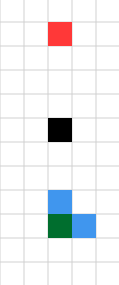
\includegraphics[scale=0.6, height =4cm]{Bilder/pathfinding_procedure_2.png}
					\subcaption{2. Feld durchlaufen}
					\label{pic:pathpro2}
				\end{subfigure}%
				\qquad
				\begin{subfigure}[h]{.17\linewidth}
					\centering
					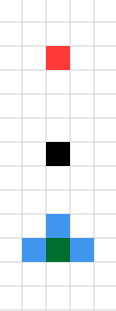
\includegraphics[scale=0.6, height =4cm]{Bilder/pathfinding_procedure_3.png}
					\subcaption{3. Feld durchlaufen}
					\label{pic:pathproc3}
				\end{subfigure}%
				\qquad % erzeugt etwas Abstand
				\begin{subfigure}[h]{.17\linewidth}
					\centering
					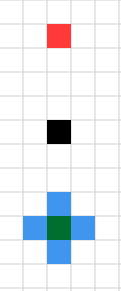
\includegraphics[scale=0.6, height =4cm]{Bilder/pathfinding_procedure_4.png}
					\subcaption{4. Feld durchlaufen}
					\label{pic:pathproc4}
				\end{subfigure}%
				\caption{Funktionsweise eine Pathfinding-Algorithmus}
				\label{pic:pathproc}
			\end{figure}
			
			
			%evtl \newpage
			Dies wird in Abbildung \ref{pic:pathproc}verdeutlicht. Grün repräsentiert den Startpunkt, Rot den Endpunkt. Schwarz repräsentiert ein nicht passierbares Feld und blaue Felder sind von dem Suchalgorithmus bereits besucht worden. 
			Die dargestellte Suchart stellt den \emph{Breadth-first Search Algorithmus} dar, welche zur oben gegebenen Beschreibung passt. Dabei handelt es sich um einen einfachen Wegfindungsalgorithmus.
			
			\begin{figure}[H]
				\captionsetup{width=.8\linewidth}
				\centering
				\begin{subfigure}[h]{.33\linewidth}
					\centering
					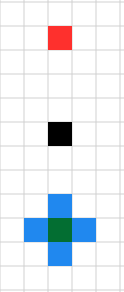
\includegraphics[scale=0.6, height =5cm]{Bilder/pathfinding_tiefe1.png}
					\subcaption{1. Feld durchlaufen}
					\label{pic:pathtiefe1}
				\end{subfigure}%
				\qquad % erzeugt etwas Abstand
				\begin{subfigure}[h]{.33\linewidth}
					\centering
					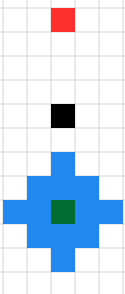
\includegraphics[scale=0.6, height =5cm]{Bilder/pathfinding_tiefe2.png}
					\subcaption{2. Feld durchlaufen}
					\label{pic:pathtiefe2}
				\end{subfigure}
				\caption{Funktionsweise eine Pathfinding-Algorithmus}
				\label{pic:pathtiefe}
			\end{figure}	
			
			Zur Verbesserung der Effizienz nutzen manche Algorithmen andere Methoden, die Schätzalgorithmen, welche man auch Heuristik nennt, die Einfluss darauf nehmen, welche Felder als nächstes besucht werden. Felder, welche in Richtung des Ziels zeigen bzw. sehr wahrscheinlich dorthin führen, werden bevorzugt durchlaufen, Felder, welche vom Ziel weg zeigen, werden hingegen seltener Besucht. Dazu misst der Algorithmus nicht nur die Distanz (Kosten) bis zu einem Punkt, um zu berechnen, ob es sich lohnt, von diesem aus weiter zu suchen, sondern auch die Distanz zum Ziel. Mathematisch kann man dies als zusammengesetzte Funktion verstehen.
			\begin{equation}
				f(x) = g(x) + h(x)
			\end{equation}
			
			Hierbei stellt $g(x)$ die Funktion dar, welche die Kosten(Distanz) vom Startpunkt bis zu einem Punkt $x$ berechnet. $h(x)$ beschreibt die vermutete Distanz von $x$ bis zum Zielpunkt. Beide Ergebnisse zusammen ergeben einen Wert, welcher die Kosten über einen Punkt $x$ zum Zielpunkt errechnet. Dies wird für viele Punkte $x$ berechnet, wobei der nächste Schritt von dem Punkt ausgeht, welcher den niedrigsten Wert (also die geringste, errechnete Distanz) hat.
			Diese Algorithmen sind für viele Verwendungszwecke sehr effizient. Heuristik nutzende Wegfindungsalgorithmen können unter Umständen nachteilig sein, wenn diese in Labyrinthen eingesetzt werden, welche eine hohe Komplexität aufweisen, da Sackgassen, welche nur durch eine Wand vom Ziel getrennt werden, meist durchsucht werden, obwohl sie im Endeffekt nicht Zielführend sind.
			
			\begin{figure}[H]
				\centering
				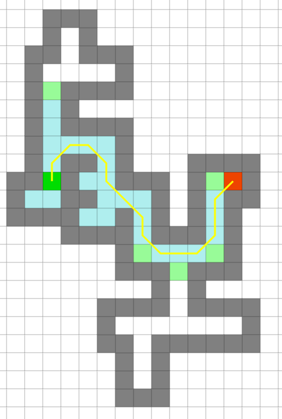
\includegraphics[height=5cm]{Bilder/pathfinding_laby_heu.png}
				\caption{Wegfindung eines Algorithmus mit Heuristik} 
				\label{pic:pathlabheu}
			\end{figure}
		
		
		
		
			\subsubsection{Costmap}
			{
				Die gegebene Karte wird in eine Costmap umgewandelt. Dabei bleibt die Grundfunktion bestehen. Eine Karte, welche Hindernisse aufzeigt. Zusätzlich dazu unterstützt diese Karte jedoch bei der Wegfindung. Jeder Punkt auf der Karte erhält einen Wert - dessen Kosten, welche die Wahrscheinlichkeit eines Zusammenstoßes beschreibt. Sind diese Kosten hoch, bedeutet dies, dass, sofern der Mittelpunkt des Roboters sich auf diesem Punkt befindet, eine Kollision mit einem Gegenstand sehr wahrscheinlich ist. Je weiter ein Punkt von einem Hindernis entfernt ist, desto geringer ist der Wert dieses Punktes. 
				\begin{figure}[H]
					\centering				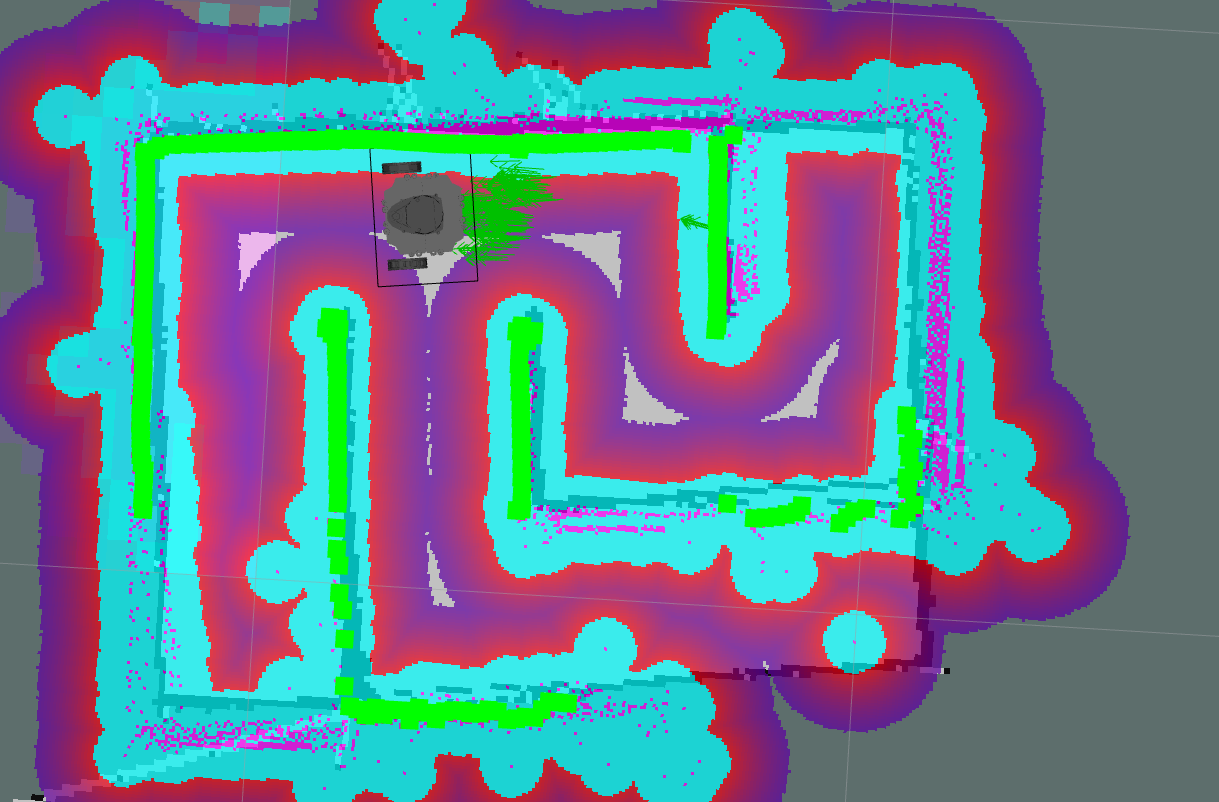
\includegraphics[height=5cm]{Bilder/costmap_overlayed.png}
					\caption{Die Costmap einer Karte} 
					\label{pic:costmapoverlayed}
				\end{figure}
				Abbildung \ref{pic:costmapoverlayed} zeigt die Costmap. Es ist zu erkennen, dass der Bereich um Hindernisse (lila) verschieden gefärbt ist, was die abnehmenden Kosten für diesen Punkt beschreibt.
			}
			
			\subsubsection{Wegplanung}
			{
				Der zu befahrende Weg wird basierend auf mehreren Variablen geplant. Dazu zählt die Distanz im groben, \dahe der kürzeste Weg wird bevorzugt, aber auch gleichzeitig die Wahrscheinlichkeit einer Kollision während des Weges. Dazu werden die Kosten der Punkte auf der Costmap, welche auf dem Weg liegen betrachtet. Um mehr Variabilität bei der Wegplanung zu erlauben, wird die Planung in zwei Bereiche unterteilt. Ein globaler Planer plant den groben Weg zum Ziel, während ein lokaler Planer den Weg entlang des groben Weges plant, wobei gegebenenfalls auch Korrekturen vorgenommen werden müssen.
				
				\begin{figure}[H]
					\centering				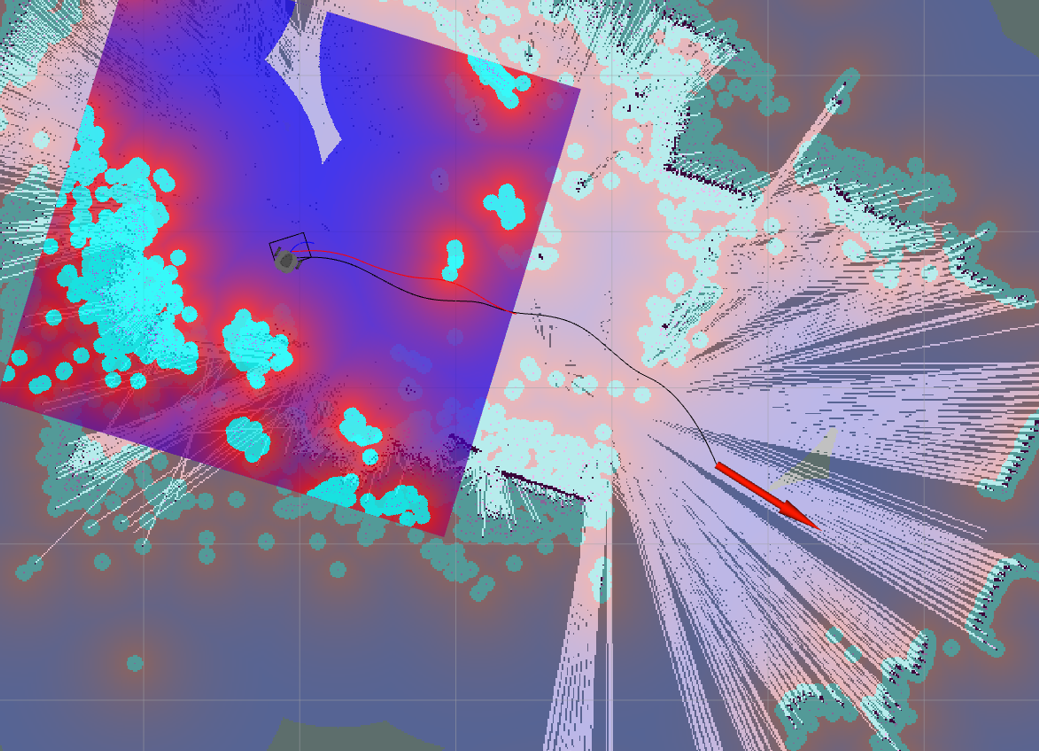
\includegraphics[height=5cm]{Bilder/costmap_pathplanning.png}
					\caption{Die Wegplaning, visualisiert in Rviz} 
					\label{pic:costpathplanning}
				\end{figure}
				
				Die obige Abbildung visualisiert den geplanten Weg. Dieser ist in einen roten, den lokal geplanten Weg, sowie einen Schwarzen, den global geplanten Weg aufgeteilt. Der blaue Strich repräsentiert die momentane Bewegungsrichtung. Weiter ist zu erkennen, dass die Costmap in einen lokalen Bereich (Rechteck), sowie einen globalen Bereich, welcher die ganze Karte umfasst, hat. Der lokale Bereich ist für die kurzfristige Wegplanung (lokaler Planer) für Bedeutung und hebt Hindernisse stärker hervor.
				
			}
			\subsection{Die move\tus base} %https://www.researchgate.net/publication/253239158_ROSoClingo_A_ROS_package_for_ASP-based_robot_control
			{
				Das move\tus base - Paket steuert die Navigation des Roboters, sowie den Pfad, welchem der Roboter folgen soll. Es besteht aus mehreren Nodes (in Abbildung \ref{pic:overviewmovebase}oval dargestellt).  Dazu abonnieren dieser Node verschiedene Topics. Dazu gehören Sensordaten (z.B. \emph{sensor\textunderscore msgs/LaserScan} für die Daten des LiDAR-Sensors), Odometriedaten und eine Karte. Die Karte wird durch einen Kartenserver bereitgestellt, was aber auch der \emph{GMapping} - Node sein kann
				\begin{figure}[H]
					\centering
					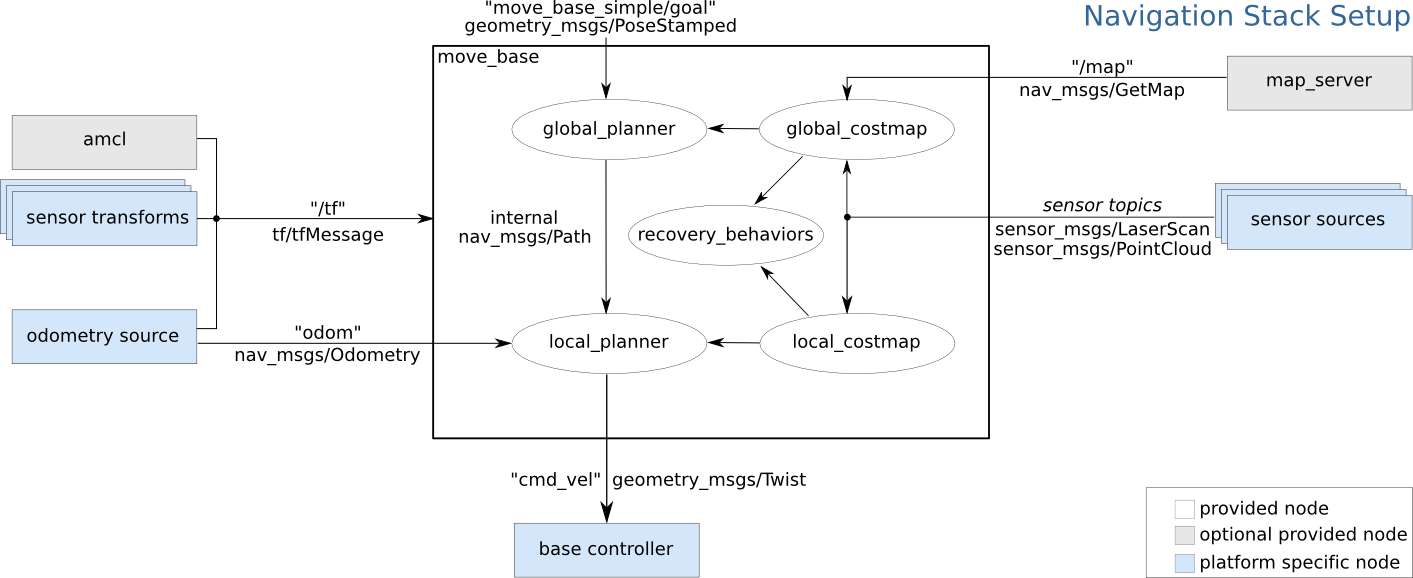
\includegraphics[height=6.5cm]{Bilder/overview_move_base.png}
					\caption{Das move\textunderscore base - Paket \\
						\parencite{movebasenodeoverview}} 
					\label{pic:overviewmovebase}
				\end{figure}
				

}
